\documentclass[aspectratio=169,fleqn,xcolor={dvipsnames}]{beamer}
%Template by Lukas

\usetheme[pageofpages=of]{hubln}
% dette dokumentet er hoveddokumentet og må kompileres
% resten skjer i Preamble.tex

\usepackage[utf8]{inputenc}
\usepackage[T1]{fontenc}
\usepackage{geometry}
\usepackage{amsmath}
\usepackage{graphicx}
\usepackage{listings}%For code do \begin{lstlisting}
\usepackage{color}
\usepackage{tikz-cd}
\usepackage{float}
\usepackage{glossaries}
\usepackage{fancyhdr}
\usepackage{cleveref}
\usepackage{epigraph}
\usepackage{tikz}
%\definecolor{bg}{HTML}{282828}
\definecolor{bg}{RGB}{40, 40, 40}
\setbeamercovered{invisible}
\hfuzz=8.64pt % Antioverfullbox-inator

\setbeamercolor{block body alerted}{bg=alerted text.fg!10}
\setbeamercolor{block title alerted}{bg=alerted text.fg!20}
\setbeamercolor{block body}{bg=structure!10}
\setbeamercolor{block title}{bg=structure!20}
\setbeamercolor{block body example}{bg=green!10}
\setbeamercolor{block title example}{bg=green!20}
\setbeamertemplate{blocks}[rounded][shadow]
\graphicspath{ {../assets/} }

\tikzset{onslide/.code args={<#1>#2}{% from https://tex.stackexchange.com/a/6155/263192
  \only<#1>{\pgfkeysalso{#2}}
}}

\newcommand{\newLine}{%
  \hfill\break
}

%\newcommand{\comment}[1]{}
\tikzset{vertex/.style={draw, circle, inner sep=1mm}}
\newcommand{\incomplete}[3][1.5cm]{\begin{tikzpicture}
\foreach \n in {1,...,#2}{\node[vertex]at({90-360/#2*(\n-1)}:#1)(\n){\n};}
\foreach \v/\w in {#3}{\draw(\v)--(\w);}
\end{tikzpicture}}
\tikzset{properties/.style={orange, ultra thick}}
\tikzset{propertiesRed/.style={red, ultra thick}}
\tikzset{propertiesBlue/.style={blue, ultra thick}}
\tikzset{propertiesGrey/.style={gray, ultra thick}}

\usepackage{mathtools}
\DeclarePairedDelimiter\ceil{\lceil}{\rceil}
\DeclarePairedDelimiter\floor{\lfloor}{\rfloor}

% Hier die Daten zur Präsentation eintragen
\author[ls]{Sander Wiig}
\title[sgp]{Crashcourse INF222}
\institute{Institutt for informatikk \\ Universitetet i Bergen}
\date[\today]

\begin{document}
  %Innholdet til selveste presentasjon
%Titel page
\begin{frame}[t,plain]
    \titlepage
\end{frame}

% her kan du plassere en QR kode som lar folk laste ned filen (filene er i images folder)
\subsection*{Download the PDF}
\begin{frame}{Script and Presentation}
    \begin{figure}
        \centering
        
\includegraphics[height = 4.9cm]{qrcode.png}
        \caption{https://github.com/Swi005/Book-of-Magne/tree/v2023}
        \label{fig:qrcode}
    \end{figure}
\end{frame}

%===============================================
%Innholdet til selveste presentasjonen
\section{Programming Languages}
\subsection{What is a Programming Language?}
\begin{frame}{\textbf{What is a Programming Language?}}
    A Programming language is ...
    \begin{itemize}[<+->]
        \item used to tell a computer what to do
        \item usually artificial
    \end{itemize}
\end{frame}

\subsection{Grouping Languages by Domain}
\begin{frame}{\textbf{Grouping Languages by domain}}
    Languages are usually grouped into two categories when based on their specificity
    \begin{itemize}[<+->]
        \item DSLs, small,  targeted at specific problems. Internal/embedded vs external 
        \item GPLs, large, many uses.
    \end{itemize}
\end{frame}
\subsection*{Grouping Languages by Domain}
\begin{frame}{\textbf{Grouping Languages by domain}}
    \begin{figure}[!h]
        \centering
        \begin{tabular}{|c|c|c|c|}
            \hline
            \textbf{Characteristic} &\textbf{DSL } &\textbf{GPL}\\
            \hline
            \textbf{Domain} & Small and well-defined domain & Generality, many use cases\\
            \hline
            \textbf{Size} &Small ASTs & Large ASTs, often user extensible\\
            \hline
            \textbf{Lifespan} &As long as their domain &years to decades\\
            \hline
            \textbf{Extensibility} &Usually not extendible & Extendable\\
            \hline
        \end{tabular}%
        \caption{Comparison between GPLs and DSLs}
    \end{figure}%
\end{frame}


\subsection{Syntax and Semantics}
\begin{frame}{\textbf{Syntax and Semantics}}
    \begin{block}{Definition}
        All languages consist of two parts
        \begin{itemize}[<+->]
            \item \textbf{Syntax} - Defines shape
            \item \textbf{Semantics} - Defines meaning
        \end{itemize}
    \end{block}
    \Large
    Syntax is defined by a grammar.\\
    Grammar is not covered in this course :)
\end{frame}


\subsection{Meta Programming}
\begin{frame}{\textbf{Meta Programming}}
    A metaprogram is a program that works on \textit{other} programs.\\
    Compilers and Interpreters are examples of metaprograms
    \begin{block}{Definition}
        \begin{itemize}
            \item \textbf{Object Language} - Langage that gets compiled/interpreter
            \item \textbf{Meta Language} - Language used to implement the compiler/interpreter
        \end{itemize}
    \end{block}
\end{frame}

\subsection{Sum of Products}
\begin{frame}[fragile]{\textbf{Sum of Products}}
    \begin{figure}
        \centering
        \begin{minipage}{.5\textwidth}
            \begin{lstlisting}[language=Haskell]
    data SomeType = A Bool Bool Bool
                    | B Bool
                    | C
            \end{lstlisting}
        \end{minipage} 
    \end{figure}
    
    \begin{examples}
        \begin{equation*}
            \underbrace{(\text{Bool} \times \text{Bool} \times \text{Bool})}_{A} + \underbrace{\text{Bool}}_{B} + \underbrace{1}_{C}
        \end{equation*}
        \texttt{Bool} is either \texttt{True} or \texttt{False}.\\
        The total number of values of type SomeType is $8 + 2 + 1 = 11$.
    \end{examples}
\end{frame}

\subsection*{Sum of Products}
\begin{frame}[fragile]{\textbf{Sum of Products}}
    \begin{figure}
        \centering
        \begin{minipage}{\textwidth}
            \centering
            \begin{lstlisting}[language=Java]
    interface SomeType {}
    class A implements SomeType {
        boolean a;
        boolean b;
        boolean c ;
    }
    class B implements SomeType {
        boolean a;
    }
    class C implements SomeType {
    }
            \end{lstlisting}
        \end{minipage}
        \caption{Sum of Products in Java}
    \end{figure}
\end{frame}

\subsection*{Q\&A}
\begin{frame}{Questions?}
    \begin{figure}
        \centering
        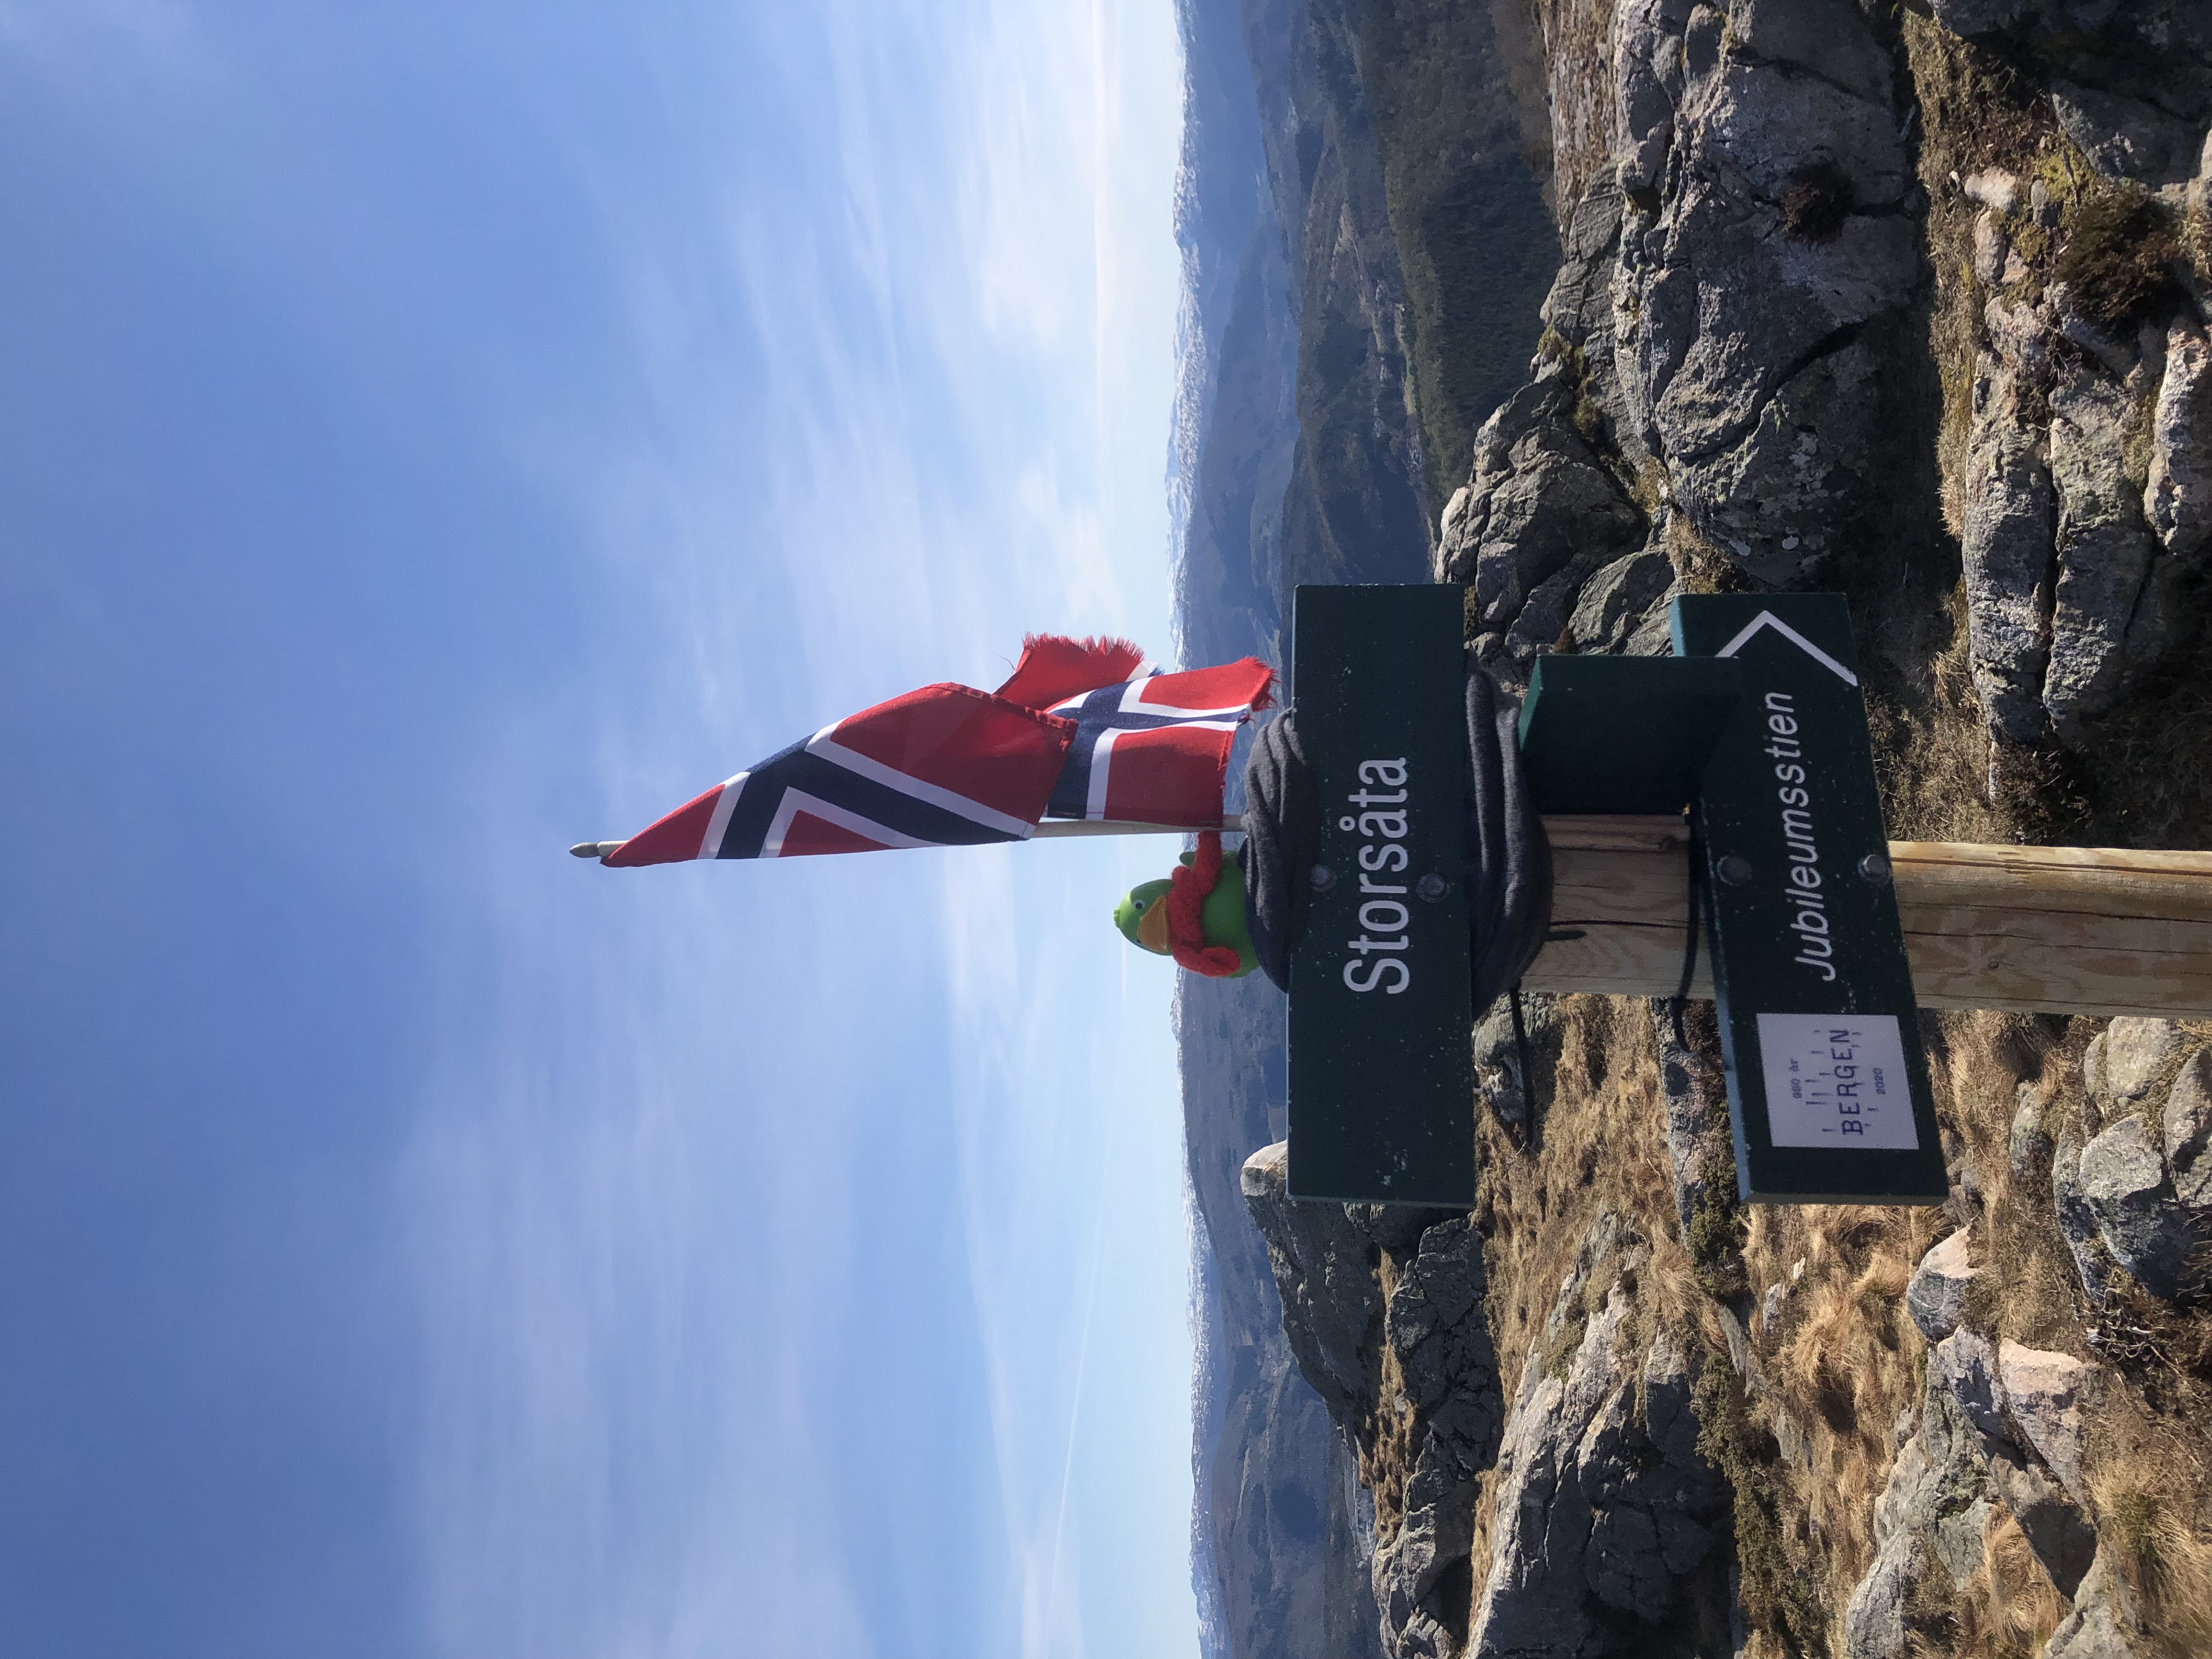
\includegraphics[height = 4.9cm]{guillaume2.jpg}
    \end{figure}
\end{frame}



\section{Interpreters}
\subsection{Compiler vs. Interpreters}
\begin{frame}{\textbf{Compiler vs. Interpreters}}
    \begin{figure}
        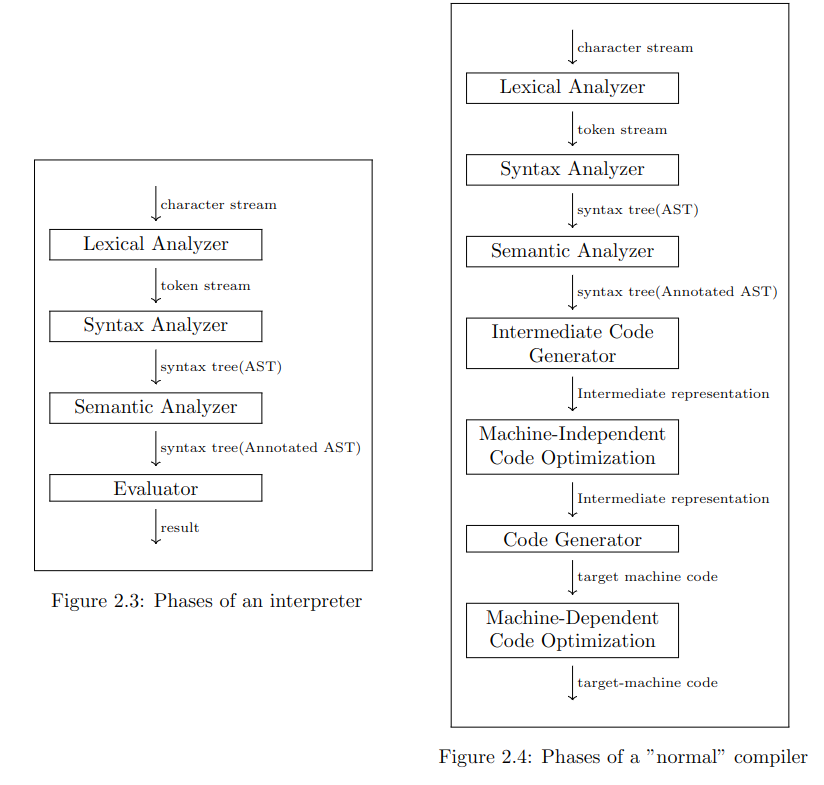
\includegraphics[scale=0.30]{Interpreter vs. Compiler.png}   
    \end{figure}
\end{frame}


\begin{frame}{\textbf{NB! IMPORTANT}}
    \begin{alertblock}{Compilers vs Interpreters!}
        We often end up using the term Compiler to talk about both Compilers and Interpreters, this is because they are very similar.\\
        This course deals exclusively with interpreters so unless stated otherwise assume that we are talking about interpreters.
    \end{alertblock}
    \begin{alertblock}{Expr vs AST}
        \begin{itemize}
            \item \textbf{Expr}: Expressions are terms that can be evaluated to a value, e.g. \texttt{1+2*3}
            \item \textbf{Stmt}: Statements are terms that are executed and result in a change of state. e.g. \texttt{var a = 1+2*3}
        \end{itemize}
    \end{alertblock}
\end{frame}

\subsection{Phases of an Interepreter}
\begin{frame}[fragile]{\textbf{Lexical Analysis}}
    \begin{block}{}
        \textbf{Lexical Analysis} breaks up strings into tokens. Also called a tokenizer.
    \end{block}
    \begin{example}
        \begin{figure}
            \centering
            \Large
            \begin{align*}
                (1+2)*13
            \end{align*}
        \end{figure}
        This gets tokenized into 
        \begin{lstlisting}[language=Haskell]
    ["(","1","+",2",")","*","13"]
        \end{lstlisting}
    \end{example}
\end{frame}
\subsection*{Phases of an Interepreter}
\begin{frame}{\textbf{Syntax Analyser}}
    \begin{example}
        \begin{figure}
            \centering
            \adjustbox{scale=0.7,center}{%
            \begin{tikzcd}
                \node[] (e0) {expr};
                \node[below left = of e0] (e1) {expr};
                \node[below left = of e1] (e11) {"("};
                \node[below = of e1] (e12) {expr};
                \node[below right = of e1] (e13) {")"};
                \node[below left = of e12] (e121) {number};
                \node[below = of e121] (e1211) {"1"};
                \node[below = of e12] (e122) {"+"};
                \node[below right = of e12] (e123) {number};
                \node[below = of e123] (e1231) {"2"};
                \node[below = of e0] (e2) {"*"};
                \node[below right = of e0] (e3) {number};
                \node[below = of e3] (e31) {"13"};
        
                \draw (e0) edge (e1)
                    (e0) edge (e2)
                    (e0) edge (e3)
                    (e1) edge (e11)
                    (e1) edge (e12)
                    (e1) edge (e13)
                    (e12) edge (e121)
                    (e12) edge (e122)
                    (e12) edge (e123)
                    (e121) edge (e1211)
                    (e123) edge (e1231);
        
            \end{tikzcd}
            }
        \end{figure}
    \end{example}
\end{frame}

\begin{frame}{\textbf{AST}}
    \begin{example}
        \begin{figure}[!h]
            \centering
            \adjustbox{scale=1,center}{%
            \begin{tikzcd}
                \node[] (e0) {\texttt{Mult}};
                \node[below left = of e0] (e1) {\texttt{Add}};
                \node[below left = of e1] (e11) {\texttt{1}};
                \node[below right = of e1] (e12) {\texttt{2}};
                \node[below right = of e0] (e2) {\texttt{13}};
        
                \draw (e0) edge (e1)
                    (e0) edge (e2)
                    (e1) edge (e11)
                    (e1) edge (e12);
            \end{tikzcd}
            }
        \end{figure}
    \end{example}
\end{frame}

\subsection{Semantic Analysis}
\begin{frame}{\textbf{Semantic Analyisis}}
    Semantic analysis lets us find out if the program is wellformed at find bugs at compile time, instead of at runtime.
    It also annotates the AST with certain information that's necessary for execution.

    \begin{block}{Wellformedness}
        For a program to be wellformed, we need to check for the following:
        \begin{itemize}
            \item \textbf{Type correctness}: The types of expressions in the program are correct.
            \item \textbf{Scope correctness}: The variables used in the program are declared.
            \item \textbf{Flow correctness}: The program is not stuck in an infinite loop.
            \item and more\dots
        \end{itemize}
        The first point is checked by a \textbf{type checker}.
    \end{block}
\end{frame}

\subsection{Type Checking}
\begin{frame}[fragile]{\textbf{Type Checking}}
    
    \begin{example}
        AST
        \lstinputlisting[language=Haskell, firstline=2, lastline=11]{examples/typecheck/typecheck.hs}
    \end{example}
\end{frame}
\subsection*{Type Checking}
\begin{frame}[fragile]{\textbf{Type Checking}}
    \begin{example}
        Types
        \lstinputlisting[language=Haskell, firstline=12, lastline=12]{examples/typecheck/typecheck.hs}
    \end{example}
\end{frame}

\begin{frame}[fragile]{\textbf{Type Checking}}
    \begin{example}
        \lstinputlisting[language=Haskell, firstline=14, lastline=21]{examples/typecheck/typecheck.hs}
    \end{example}
\end{frame}

\begin{frame}[fragile]{\textbf{Type Checking}}
    \begin{example}
        \lstinputlisting[language=Haskell, firstline=23, lastline=26]{examples/typecheck/typecheck.hs}
    \end{example}
\end{frame}

\begin{frame}[fragile]{\textbf{Type Checking}}
    \begin{example}
        \lstinputlisting[language=Haskell, firstline=28, lastline=31]{examples/typecheck/typecheck.hs}
    \end{example}
\end{frame}

\begin{frame}[fragile]{\textbf{Type Checking}}
    \begin{example}
        \lstinputlisting[language=Haskell, firstline=33, lastline=36]{examples/typecheck/typecheck.hs}
    \end{example}
\end{frame}

\begin{frame}[fragile]{\textbf{Type Checking}}
    \begin{example}
        \lstinputlisting[language=Haskell, firstline=38, lastline=41]{examples/typecheck/typecheck.hs}
    \end{example}
\end{frame}

\begin{frame}[fragile]{\textbf{Type Checking}}
    \begin{example}
        \lstinputlisting[language=Haskell, firstline=43, lastline=46]{examples/typecheck/typecheck.hs}
    \end{example}
\end{frame}

\begin{frame}[fragile]{\textbf{Type Checking}}
    \begin{example}
        \lstinputlisting[language=Haskell, firstline=48, lastline=48]{examples/typecheck/typecheck.hs}
    \end{example}
\end{frame}

\begin{frame}[fragile]{\textbf{Type Checking}}|
    \begin{example}
        \lstinputlisting[language=Haskell, firstline=50]{examples/typecheck/typecheck.hs}
    \end{example}
\end{frame}
\subsection*{Q\&A}
\begin{frame}{Questions?}
    \begin{figure}
        \centering
        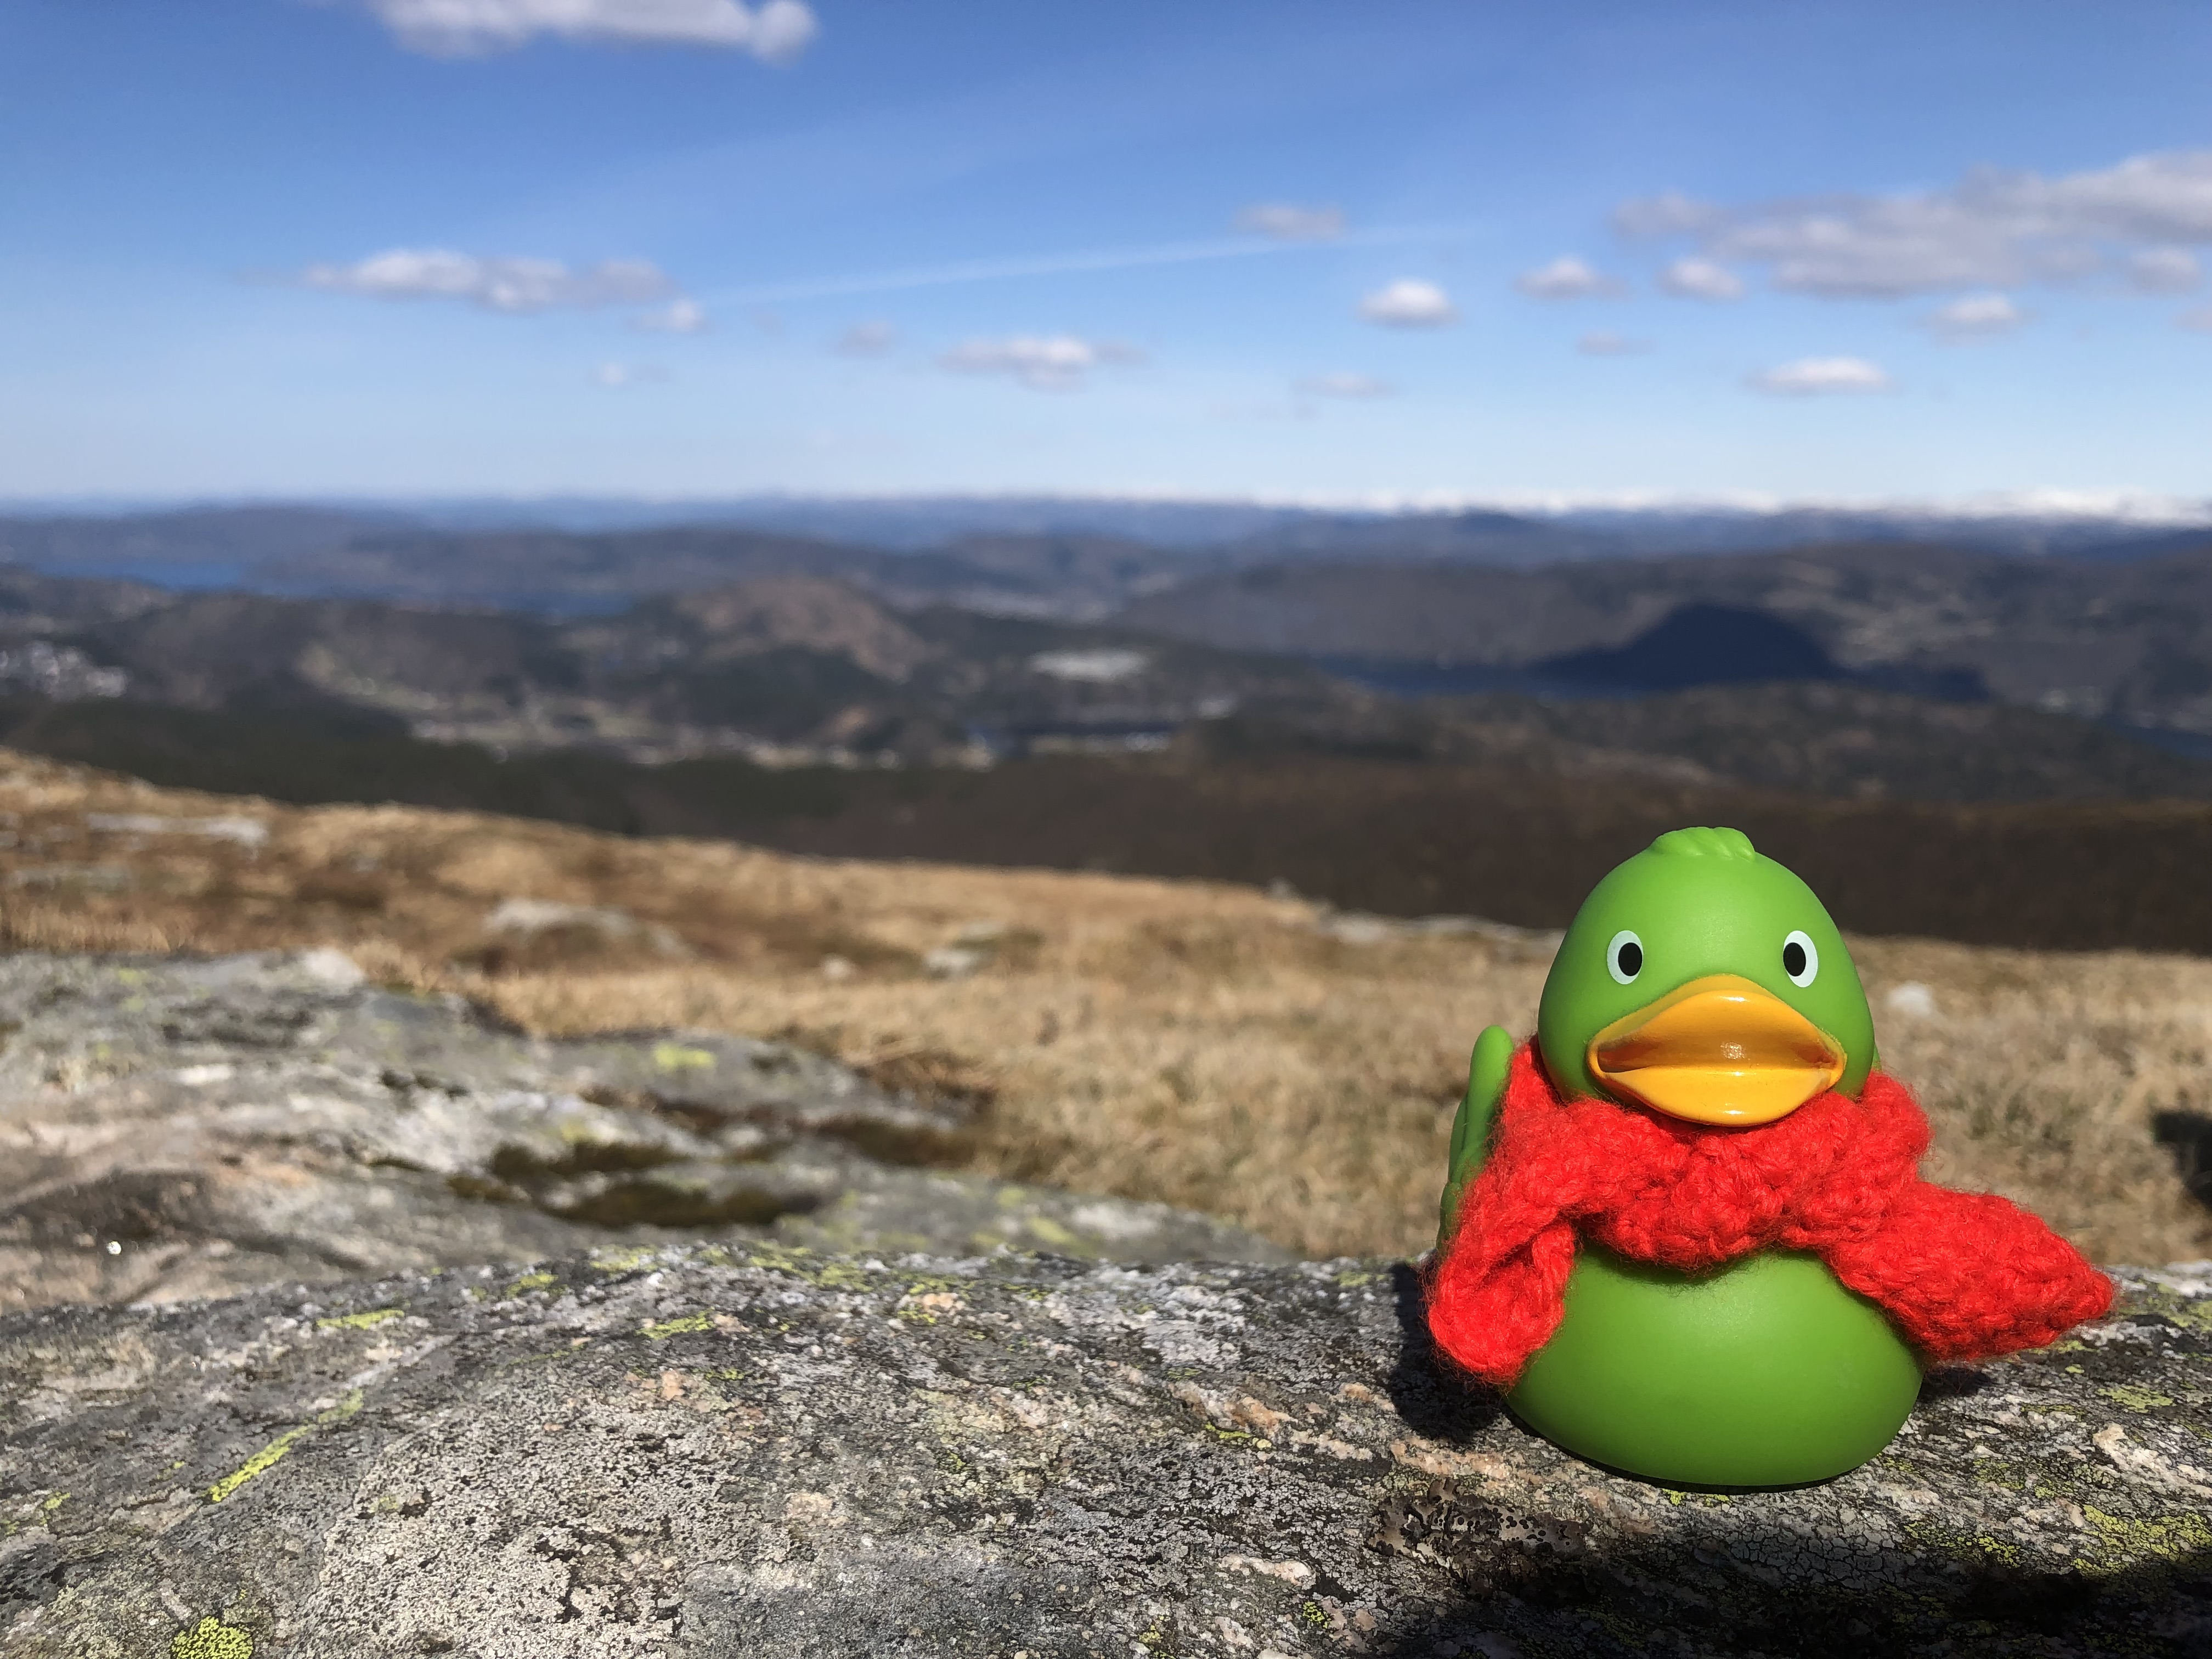
\includegraphics[height = 4.9cm]{guillaume3.jpg}
    \end{figure}
\end{frame}

\subsection*{Compiler vs. Interpreters}
\subsection{Phases of an Interepreter}
\subsubsection{Lexical Analyzer}
\subsubsection*{Static analyzer}
\subsubsection*{Semantic Analyzer}
\subsubsection*{Evaluator}
\subsection*{ASTs}
\subsection*{Type Checking}
\subsection*{Wellformedness}

\section{State}
\subsection*{Enviroment}
\subsection*{Store}
\subsection*{Scoping}
\subsection*{Storage}
\subsubsection*{Arrays}
\subsubsection*{Multiarrays}
\subsubsection*{Records}


\section{Procedures}

\subsection*{What is a Procedure}
\begin{frame}{\textbf{What is a Procedure}}
    \begin{itemize}
        \item Procedures are "programs within programs"
        \item Procedures have their own environment
    \end{itemize}
    \begin{alertblock}{Functions vs. Procedures}
        \begin{equation}
            \text{Functions} \neq \text{Procedures}
        \end{equation}
        Functions are expressions, procedures are statements.\\
        Very often same implementation.
    \end{alertblock}
\end{frame}

\subsection*{Anatomy of a procedure}
\begin{frame}{\textbf{Anatomy of a Procedure}}
    \begin{figure}
        \lstinputlisting[language=Pascal]{examples/anatomy.pipl}
    \end{figure}
    \begin{block}{Params}
        \begin{itemize}
            \item \textbf{OBS} - "read only"
            \item \textbf{UPD} - "read/write"
            \item \textbf{OUT} - "write only"
        \end{itemize}
    \end{block}
\end{frame}

\begin{frame}{\textbf{Declaration vs. Calling}}
    \begin{figure}
        \lstinputlisting[language=pascal, basicstyle=\ttfamily\tiny]{examples/ex1.pipl}
        \label{fig:ex1}
        \caption{Swap Procedure}
    \end{figure}
\end{frame}

\subsection*{Paramter Semantics}
\begin{frame}{\textbf{Parameter Semantics}}
    \Large
    Two types of parameter semantics:
    \begin{itemize}
        \item Reference semantics
        \item Copy semantics
    \end{itemize}
\end{frame}

\begin{frame}{\textbf{Reference Semantics}}
    \Large
    \begin{itemize}
        \item Parameters become aliased to arguments 
        \item Points to same memory address
        \item Unsafe, but sometimes useful
    \end{itemize}
\end{frame}
\begin{frame}{\textbf{Running a procedure with reference semantics}}
    \Large
    \begin{enumerate}[<+->]
        \item Get stackframe
        \item Wipe environment
        \item Add parameters to the environment with same address as arg
        \item run the procedure code
        \item restore the environment
    \end{enumerate}
\end{frame}
\begin{frame}{\textbf{Copy Semantics}}
    \Large
    \begin{itemize}
        \item Parameters are declared as variables and initialized with args' value
        \item Safer
        \item More intuitive behavior
        \item More complicated to implement
    \end{itemize}
\end{frame}

\begin{frame}{\textbf{Running a procedure with copy semantics}}
    
    \begin{enumerate}[<+->]
        \item Get stackframe
        \item Get values of args
        \item Wipe environment
        \item Add parameters to environment
        \item init those parameters with the arg values
        \item run the procedure code
        \item get the values of the parameters
        \item restore the environment
        \item copy the parameter values back to the args
    \end{enumerate}
\end{frame}


\subsection*{Reference semantics!}
\begin{frame}\textbf{{Reference semantics}}
    \lstinputlisting[language=Pascal]{examples/paramater semantics/copy/paramsem.pipl}
\end{frame}
\begin{frame}\textbf{{Reference semantics}}
    \lstinputlisting[language=Pascal]{examples/paramater semantics/copy/paramsem1.pipl}
\end{frame}
\begin{frame}\textbf{{Reference semantics}}
    \lstinputlisting[language=Pascal]{examples/paramater semantics/copy/paramsem2.pipl}
\end{frame}
\begin{frame}\textbf{{Reference semantics}}
    \lstinputlisting[language=Pascal]{examples/paramater semantics/copy/paramsem3.pipl}
\end{frame}

\subsection*{Example!}
\begin{frame}{\textbf{Swap example v2}}
    \lstinputlisting[language=Pascal]{examples/paramater semantics/paramsem.pipl}
\end{frame}

\subsection*{Copy semantics!}
\begin{frame}\textbf{{Copy semantics}}
    \lstinputlisting[language=Pascal]{examples/paramater semantics/reference/paramsem.pipl}
\end{frame}

\begin{frame}\textbf{{Copy semantics}}
    \lstinputlisting[language=Pascal]{examples/paramater semantics/reference/paramsem1.pipl}
\end{frame}
\begin{frame}\textbf{{Copy semantics}}
    \lstinputlisting[language=Pascal]{examples/paramater semantics/reference/paramsem2.pipl}
\end{frame}
\begin{frame}\textbf{{Copy semantics}}
    \lstinputlisting[language=Pascal]{examples/paramater semantics/reference/paramsem3.pipl}
\end{frame}




%\section*{Slutt}
\subsection*{Q\&A}
\begin{frame}{Questions?}
    \begin{figure}
        \centering
        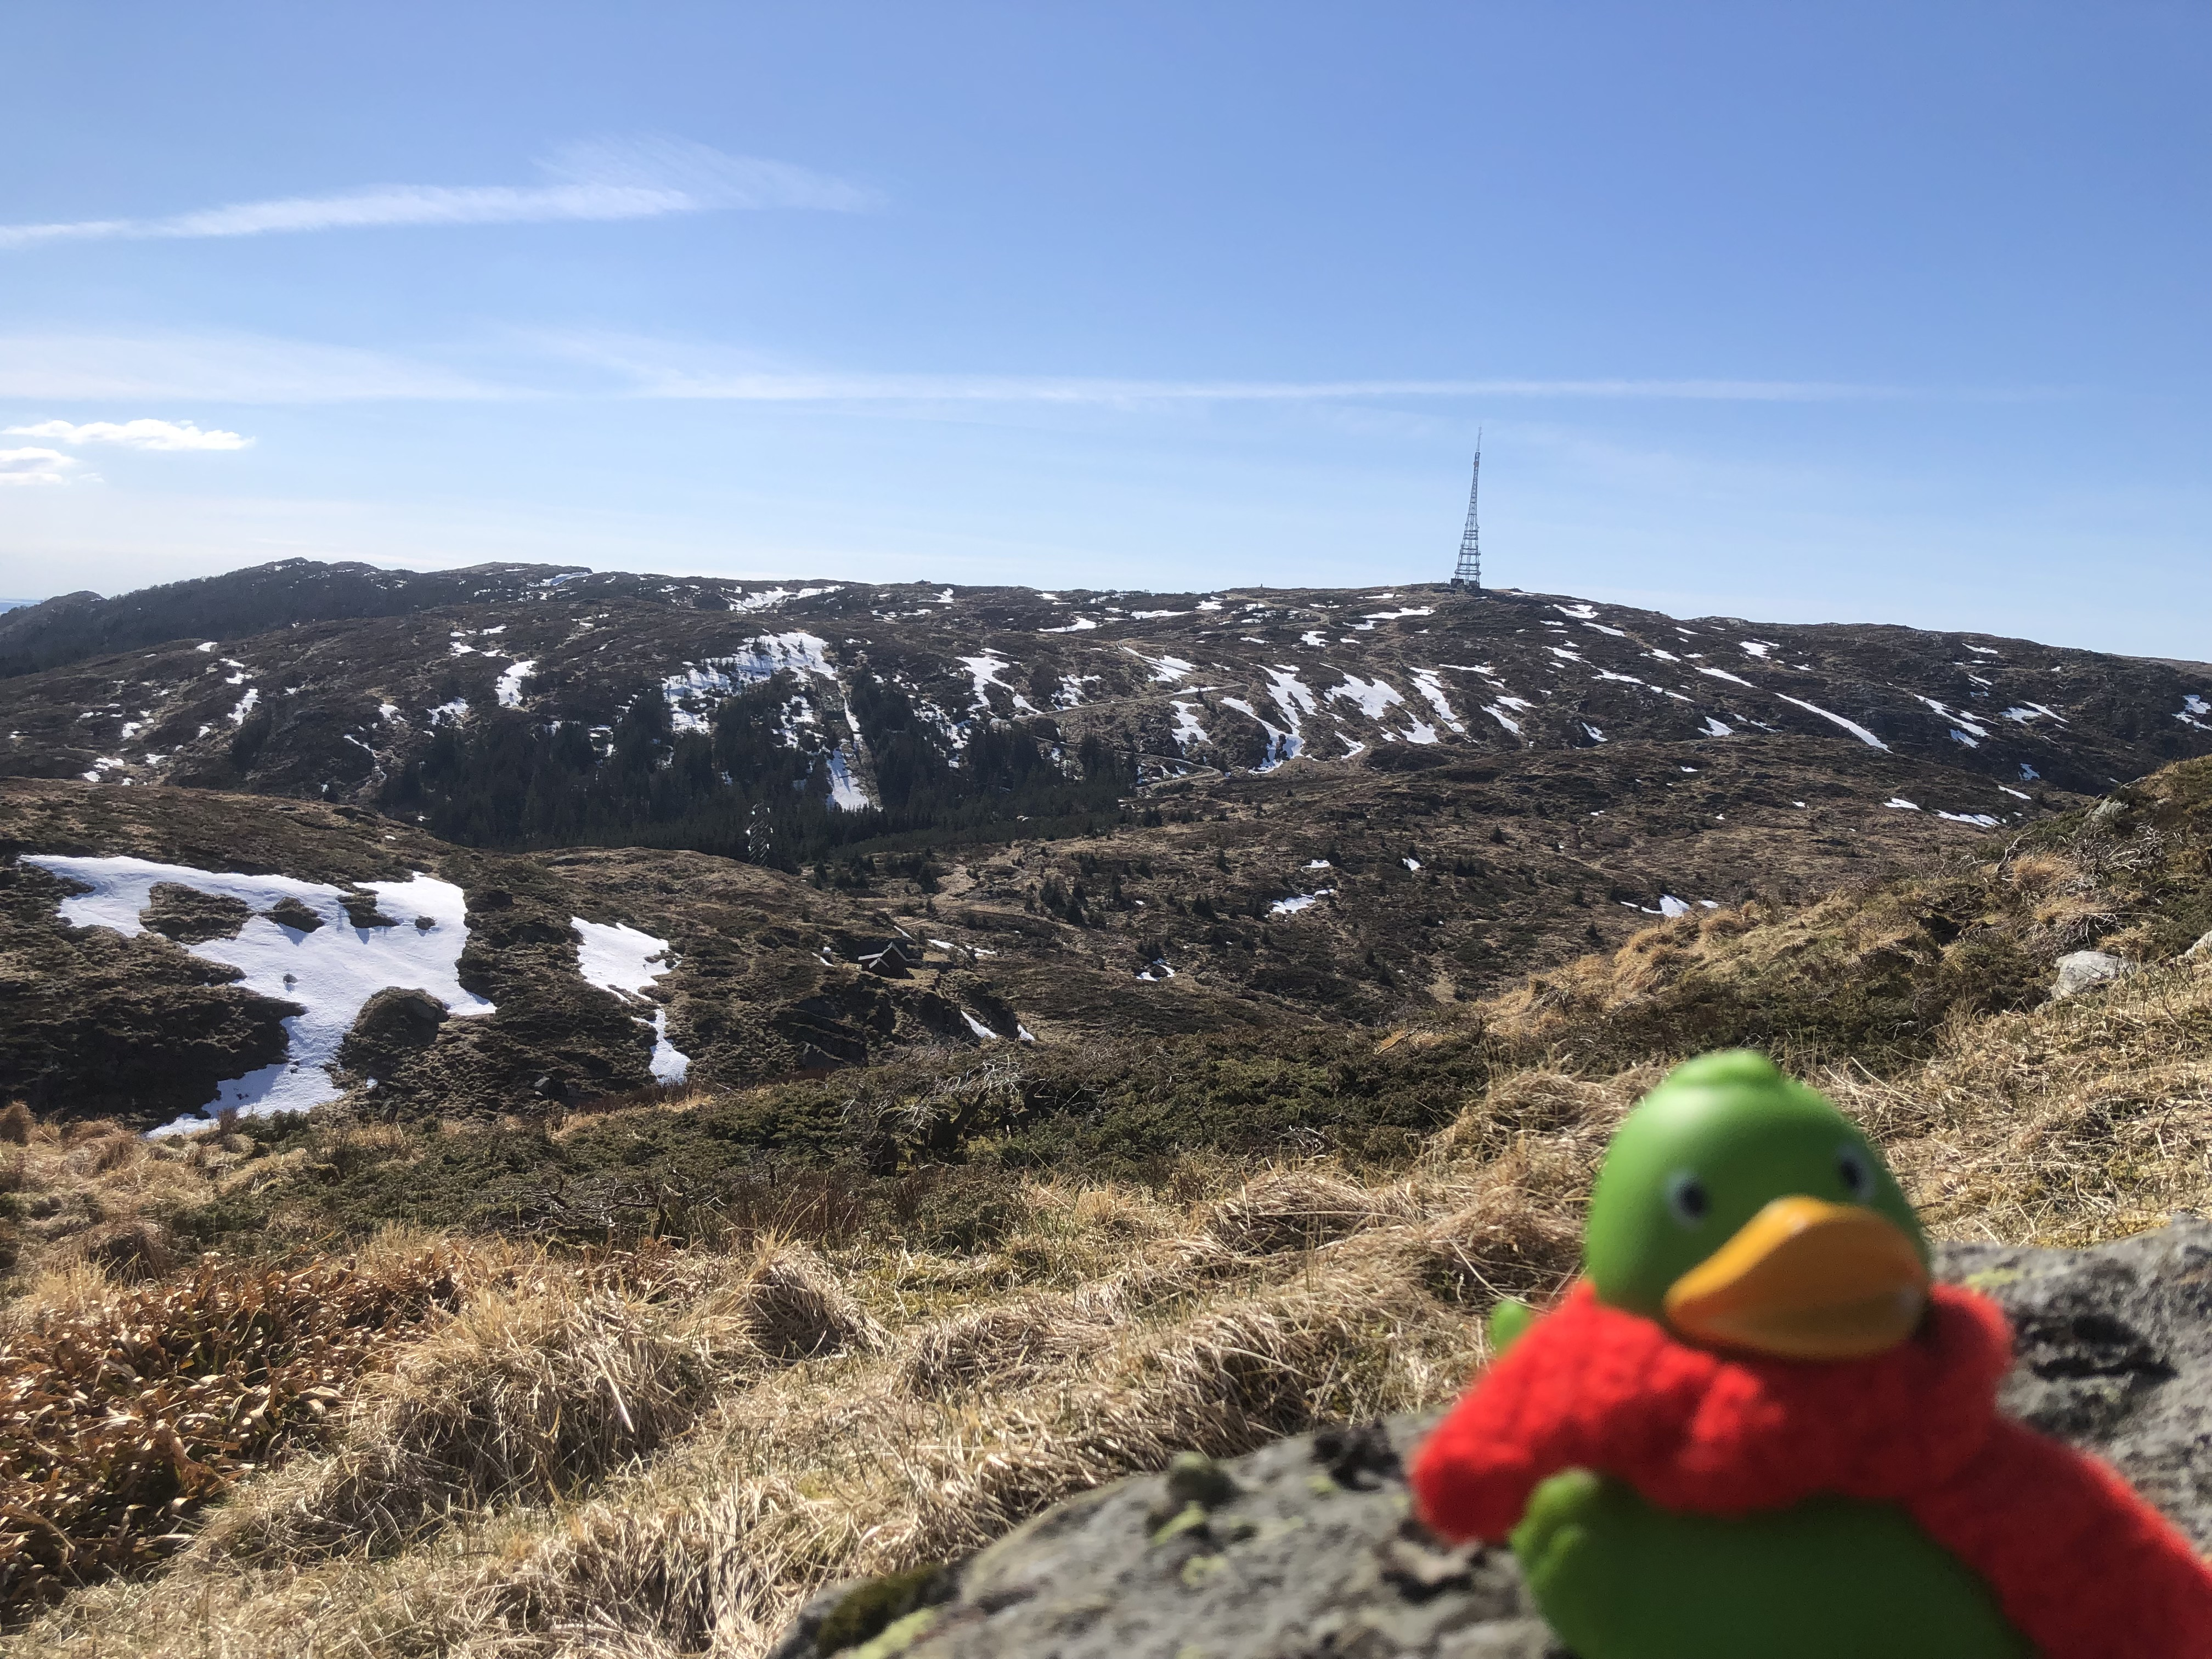
\includegraphics[height = 4.9cm]{guillaume5.jpg}
    \end{figure}
\end{frame}


\section{Signatures}
\subsection*{Signatures \& Algebras}
\subsection*{Implementing Signatures}
\subsection*{ADT's}
\subsection*{Generics}

\section{Appendix}
\subsection*{Assertions}
\subsection*{Language Standards}

\end{document}